\documentclass[12pt,a4paper,onecolumn]{article}

%%%%%%%%%%%%%%%%%%%%%%%%%%%%%%%%%%%
%          				PACKAGES  				              %
%%%%%%%%%%%%%%%%%%%%%%%%%%%%%%%%%%%

\usepackage[margin=1in]{geometry}
\usepackage{authblk}
\usepackage[utf8]{inputenc}
\usepackage{amsfonts}
\usepackage{a4wide,graphicx,color}
\usepackage{amsmath}
\usepackage{amssymb}
\usepackage[table]{xcolor}
\usepackage{setspace}
\usepackage{booktabs}
\usepackage{dcolumn}
\usepackage{rotating}
\usepackage{color,soul}
\usepackage{threeparttable}
\usepackage[capposition=top]{floatrow}
\usepackage[labelsep=period]{caption}
\usepackage[spanish]{babel}
\usepackage{subcaption}
\usepackage{lscape}
\usepackage{pdflscape}
\usepackage{multicol}
\usepackage[bottom]{footmisc}
\setlength\footnotemargin{5pt}
\usepackage{longtable} %for long tables

\usepackage{enumerate}
\usepackage{units}  %nicefraction
\usepackage{placeins}
\usepackage{booktabs,multirow}
%% BibTeX settings
\usepackage{natbib}
\bibliographystyle{apalike}
%\bibliographystyle{unsrtnat}
\bibpunct{(}{)}{,}{a}{,}{,}


%% paragraph formatting
\renewcommand{\baselinestretch}{1}


% Defines columns for tables
\usepackage{array}
\newcolumntype{L}[1]{>{\raggedright\let\newline\\\arraybackslash\hspace{0pt}}m{#1}}
\newcolumntype{C}[1]{>{\centering\let\newline\\\arraybackslash\hspace{0pt}}m{#1}}
\newcolumntype{R}[1]{>{\raggedleft\let\newline\\\arraybackslash\hspace{0pt}}m{#1}}

\usepackage{comment} %to comment entire sections



\usepackage{bbold} %for indicators

\setcounter{secnumdepth}{6}  %To get paragraphs referenced 

\usepackage{titlesec} %subsection smaller
\titleformat*{\subsection}{\normalsize \bfseries} %subsection smaller
%\usepackage[raggedright]{titlesec} % for sections does not hyphen words


\usepackage[colorlinks=true,linkcolor=black,urlcolor=blue,citecolor=blue]{hyperref}  %Load last
%% markup commands for code/software
\let\code=\texttt
\let\pkg=\textbf
\let\proglang=\textsf
\newcommand{\file}[1]{`\code{#1}'}
\newcommand{\email}[1]{\href{mailto:#1}{\normalfont\texttt{#1}}}
\urlstyle{same}

%%%%%%%%%%%%%%%%%%%%%%%%%%%%%%%%%%%
%     			TITLE, AUTHORS AND DATE    			  %
%%%%%%%%%%%%%%%%%%%%%%%%%%%%%%%%%%%
%% Title, authors and date

\title{PS1 }

\author{Catalina Leal Rojas, Lucas Daniel Carrillo Aguirre, Lucas Eduardo Veras Costa, Maria Paula Basto Lozano} 
\date{\today}

\begin{document}



\maketitle

\thispagestyle{empty} % Leaves first page without page number

%



%%%%%%%%%%%%%%%%%%%%%%%%%%%%%%%%%%%
%    DOCUMENT    		          %
%%%%%%%%%%%%%%%%%%%%%%%%%%%%%%%%%%%




\section{Introduction} \label{sec:intro}

Here you have to position your paper, remember RAP:
\begin{enumerate}
    \item R: research question
    \item A: your answer
    \item P: positioning in the existing literature
\end{enumerate}

\section{Literature Review}

A couple of things here. First, I prefer not to have a separate section, I think it's better to have it as part of the introduction, where you can cite the papers to position yours, and also in contrasting your contribution. You can also fold this when discussion your results, so you can compare/contrast with the existing literature


If you decide to have a separate section, please be careful in relating it to your research. I encurage you to read and follow \cite{nikolov2020writing}\footnote{This is available in the \href{https://ignaciomsarmiento.github.io/teaching/Tesis.html}{course website}} excellent advice:

\begin{quote}
    {\it ``Do not title your literature review section ``literature review''! It is a bit sophomoric. Instead, integrate your discussion of previous literature under the common thread of previous work as it relates to your main thesis.  For example if your paper is ``Do Traditional Institutions Constrain Female Entrepreneurship?'' you might want to call your literature review ``Gender norms in India''. In other words, tell your readers what is in the section...''} \citep{nikolov2020writing}
\end{quote}



\section{Data}

\section{¿Trabajos semejantes pagos semejantes?}

En la estimación del diferencial salarial por género bajo el principio de 
``igual remuneración por igual trabajo'', la elección de variables de control 
es fundamental. Hemos organizado las covariables en cuatro bloques analíticos:

\begin{itemize}
    \item \textbf{Capital humano}: Incluimos edad y su cuadrado como 
    aproximación a la experiencia laboral, así como el nivel educativo más alto 
    alcanzado. Estas variables capturan diferencias en productividad potencial.

    \item \textbf{Características del empleo}: Incorporamos ocupación, tamaño 
    de la firma, tipo de relación laboral, formalidad del empleo y la antigüedad 
    en el puesto. Estos factores permiten aproximar la comparabilidad entre 
    trabajos, tal como lo exige la noción de ``igual trabajo''.

    \item \textbf{Condiciones de mercado laboral}: Se añaden controles 
    geográficos (departamento y área urbana/rural) y temporales (mes de la 
    encuesta) para absorber variaciones en salarios asociadas a diferencias 
    regionales o estacionales.

    \item \textbf{Intensidad laboral}: En las especificaciones con salarios 
    mensuales, se consideran las horas usuales de trabajo y la existencia de un 
    segundo empleo. En las especificaciones con salarios por hora, estas 
    variables se omiten deliberadamente para evitar un ajuste redundante.
\end{itemize}

La estrategia empírica consiste en estimar primero la brecha salarial sin 
controles y, posteriormente, añadir secuencialmente los bloques de covariables. 
De este modo, se puede observar cómo evoluciona el coeficiente asociado a la 
variable de género, lo que permite interpretar en qué medida el diferencial 
incondicional se explica por diferencias observables en características de los 
trabajadores y de sus empleos.

\section{Results}

Referencing tables is very easy you can do the following: In Table \ref{tab:avdiscriminationrates} ...

Citing papers is easier, for example \cite{albouy2020unlocking} shows that crime around parks. For many papers in parenthesis \cite{albouy2020unlocking,mcmillen2019more} 

\subsection{Robustness}
\section{Conclusion}





%%%%%%%%%%%%%%%%%%%%%%%%%%%%%%%%%%%
%		  References				  %
%%%%%%%%%%%%%%%%%%%%%%%%%%%%%%%%%%%

\pagebreak
\singlespacing
\bibliography{References.bib}
\pagebreak


%%%%%%%%%%%%%%%%%%%%%%%%%%%%%%%%%%%
%		  TABLES				  %
%%%%%%%%%%%%%%%%%%%%%%%%%%%%%%%%%%%
\section*{Tables and Figures}


\begin{table}[H]                                 
\footnotesize \centering                                 \begin{threeparttable}                                 \captionsetup{justification=centering}                      \caption{Overall Response Rates }                               \label{tab:avdiscriminationrates}                               \begin{tabular}{@{\extracolsep{5pt}} lcc}                       \\[-1.8ex]\hline                                  
\hline \\[-1.8ex]                                  & \multicolumn{2}{c}{\it Dependent variable:} \\                                 & \multicolumn{2}{c}{\it  Response} \\                                 \cline{2-3}\\ [-1.8ex]        
                    &\multicolumn{1}{c}{(1)}   &\multicolumn{1}{c}{(2)}   \\
\hline
Minority            &     -0.323***&               \\
                    &(-0.213,-0.412)   &               \\
African American    &               &     -0.432***\\
                    &               &(-0.312,-0.532)   \\
Hispanic/LatinX     &               &     0.7027\\
                    &               &(-0.670,0.818)   \\
\hline
 Mean Response (White)&        0.4   &        0.4   \\
\hline Gender       &         Yes   &         Yes   \\
Education Level     &         Yes   &         Yes   \\
Inquiry Order       &         Yes   &         Yes   \\
\hline Observations &      45,202   &      45,202   \\
\\[-1.8ex]\hline                          
\hline \\[-1.8ex]           
\end{tabular}      
\begin{tablenotes}[scriptsize,flushleft] 
\scriptsize                         
\item Notes: Table reports coeficients from a within-property linear regression model including controls for gender, education and order the inquiry was sent. Standard errors clustered at the CBSA Downtown/Suburb level. 90\% confidence intervals reported in parentheses.                        
\end{tablenotes}                         
\end{threeparttable}                         
\end{table}        
%

\pagebreak

\begin{figure}[H]
\caption{US Map} \label{fig:robust}
    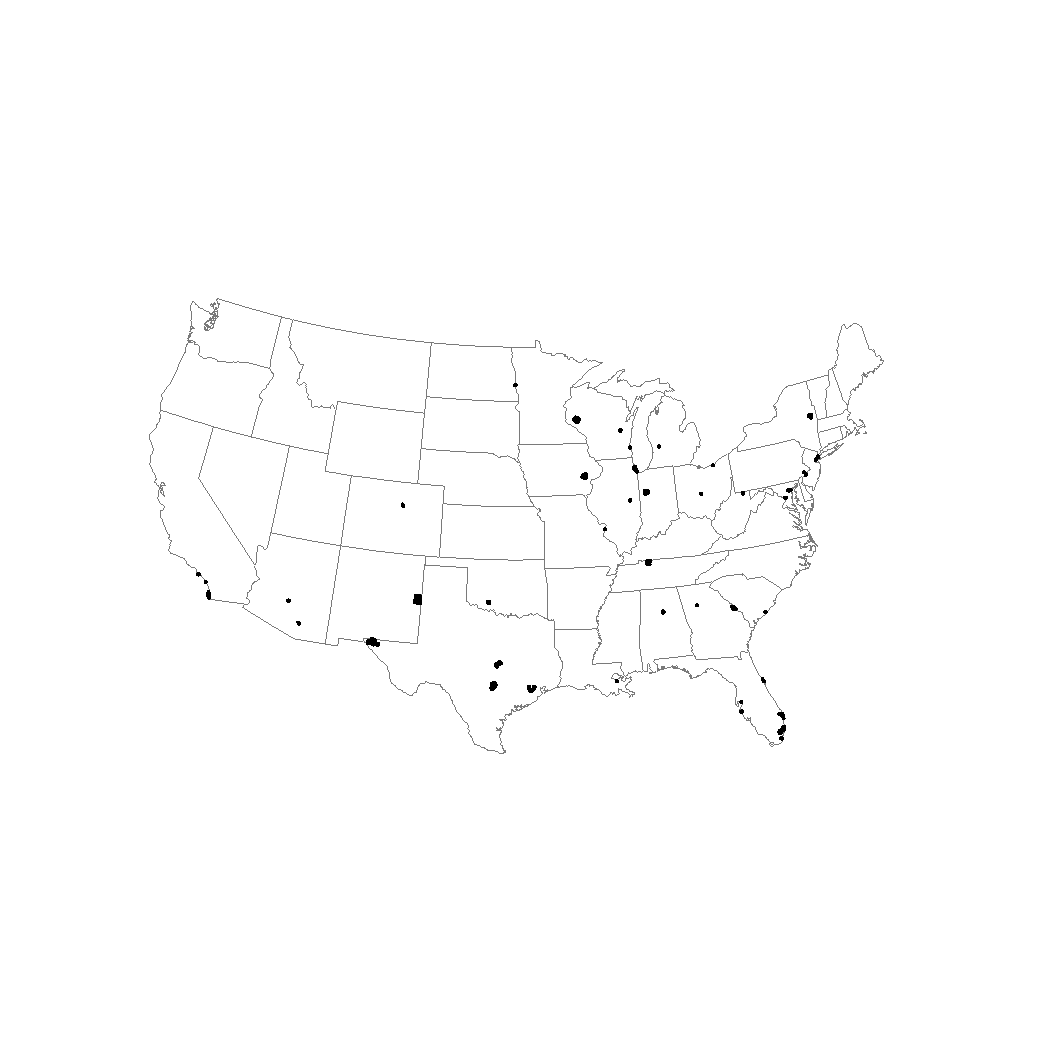
\includegraphics[scale=0.75]{../views/fig1a.pdf}   
 \flushleft
 Note: This figure shows ...
\end{figure}

%%%%%%%%%%%%%%%%%%%%%%%%%%%%%%%%
%   APPENDIX	 Tables	        %
%%%%%%%%%%%%%%%%%%%%%%%%%%%%%%%%
\pagebreak
\appendix
\renewcommand{\theequation}{\Alph{chapter}.\arabic{equation}}

\setcounter{figure}{0}
\setcounter{table}{0}
\makeatletter 
\renewcommand{\thefigure}{A.\@arabic\c@figure}
\renewcommand{\thetable}{A.\@arabic\c@table}

\section{Appendix: Tables and Figures}\label{sec:appendix_tables} 

\end{document}
